% DMA Session 11: Explorative Datenanalyse
% 180-Minuten-Block (Vorlesung + Übung interwoven)

\documentclass[usenames,dvipsnames,10pt,aspectratio=169]{beamer}
\usepackage[T1]{fontenc}
\usepackage[utf8]{inputenc}
\usepackage{verbatim}

\usetheme{ims}

\usepackage{booktabs}
\usepackage{multicol}
\usepackage{listings}
\usepackage[table]{xcolor}
\usepackage{graphicx}
\usepackage{tikz}
\usetikzlibrary{shapes.geometric, arrows.meta, positioning, calc, fit, backgrounds, matrix}
\usepackage{pifont}

% TikZ styles
\tikzset{
    tablebox/.style={rectangle, draw=IMSBlue, fill=IMSBlue!5, thick,
        minimum width=4cm, minimum height=0.8cm, font=\ttfamily\small},
    tableheader/.style={rectangle, draw=IMSBlue, fill=IMSBlue!20, thick,
        minimum width=4cm, minimum height=0.8cm, font=\ttfamily\small\bfseries},
    roadmapbox/.style={rectangle, rounded corners, minimum width=2.5cm, minimum height=0.8cm,
        text centered, draw=IMSBlue, fill=IMSBlue!10, font=\small\bfseries},
    roadmaparrow/.style={-{Stealth[length=3mm]}, thick, IMSBlue},
    sqlbox/.style={rectangle, rounded corners, draw=IMSOrange, fill=IMSOrange!10,
        minimum width=2cm, minimum height=0.6cm, font=\small},
    sqlarrow/.style={-{Stealth[length=2.5mm]}, thick, IMSOrange},
    edabox/.style={rectangle, rounded corners, minimum width=2.5cm, minimum height=1cm,
        text centered, align=center, draw=IMSBlue, thick, font=\small\bfseries, fill=IMSBlue!10},
    vizbox/.style={rectangle, rounded corners, minimum width=2.2cm, minimum height=1.5cm,
        text centered, draw=IMSOrange, thick, font=\footnotesize, fill=IMSOrange!10},
    checklistbox/.style={rectangle, rounded corners, minimum width=3.5cm, minimum height=0.6cm,
        text centered, draw=green!70!black, fill=green!10, font=\small},
    warningbox/.style={rectangle, rounded corners, minimum width=3cm, minimum height=0.8cm,
        text centered, draw=red!70, fill=red!10, font=\small},
}

% SQL Listing Style
\lstdefinestyle{sql}{
    language=SQL,
    basicstyle=\ttfamily\footnotesize,
    keywordstyle=\color{IMSBlue}\bfseries,
    stringstyle=\color{IMSOrange},
    commentstyle=\color{gray}\itshape,
    showstringspaces=false,
    breaklines=true,
    frame=single,
    backgroundcolor=\color{gray!10},
    morekeywords={SERIAL, BOOLEAN, TEXT, REFERENCES, CONSTRAINT, CASCADE, RESTRICT, PRIMARY, FOREIGN, KEY, UNIQUE, CHECK, DEFAULT, AUTO_INCREMENT, INT, VARCHAR, DATE, DECIMAL, NOT, NULL, WITH, AS, PERCENTILE_CONT, WITHIN, GROUP, OVER, PARTITION, ROWS, BETWEEN, PRECEDING, FOLLOWING, NTILE, MEDIAN, STDDEV, VARIANCE, CORR},
    literate={ü}{{\"u}}1 {ä}{{\"a}}1 {ö}{{\"o}}1 {Ü}{{\"U}}1 {Ä}{{\"A}}1 {Ö}{{\"O}}1 {ß}{{\ss}}1
}

\lstset{style=sql}

\newcommand{\cmark}{\textcolor{green!70!black}{\ding{51}}}
\newcommand{\xmark}{\textcolor{red}{\ding{55}}}
\newcommand{\pk}[1]{\underline{\texttt{#1}}}
\newcommand{\fk}[1]{\texttt{\textcolor{IMSOrange}{#1}}}

% ===== CLICKABLE AGENDA WITH PROGRESS INDICATOR =====
\usepackage{hyperref}
\hypersetup{colorlinks=false, pdfborder={0 0 0}}

% Phase counter for progress tracking
\newcounter{currentphase}
\setcounter{currentphase}{0}

% Clickable agenda item
\newcommand{\agendaitem}[3]{%
    \ifnum#1=#2
        \textcolor{IMSOrange}{$\blacktriangleright$ \textbf{\hyperlink{phase#2}{#3}}}%
    \else
        \textcolor{gray!70}{\phantom{$\blacktriangleright$} \hyperlink{phase#2}{#3}}%
    \fi\\[0.3em]%
}

% Progress dots for footline (clickable)
\newcommand{\progressdots}{%
    
\begin{tikzpicture}[baseline=-0.5ex]
        \foreach \i in {1,...,7} {
            \ifnum\value{currentphase}=\i
                \node[circle, fill=IMSOrange, minimum size=0.24cm, inner sep=0pt] at (\i*0.4,0) {\hyperlink{phase\i}{\phantom{oo}}};
            \else
                \ifnum\value{currentphase}>\i
                    \node[circle, fill=IMSBlue!60, minimum size=0.2cm, inner sep=0pt] at (\i*0.4,0) {\hyperlink{phase\i}{\phantom{oo}}};
                \else
                    \node[circle, draw=gray!50, minimum size=0.2cm, inner sep=0pt] at (\i*0.4,0) {\hyperlink{phase\i}{\phantom{oo}}};
                \fi
            \fi
        }
    \end{tikzpicture}%
}

% Add progress indicator to footline
\setbeamertemplate{footline}{%
    \leavevmode%
    \hbox{%
        \begin{beamercolorbox}[wd=.33\paperwidth,ht=2.5ex,dp=1ex,left]{author in head/foot}%
            \usebeamerfont{author in head/foot}\hspace*{2ex}\insertshortauthor
        \end{beamercolorbox}%
        \begin{beamercolorbox}[wd=.34\paperwidth,ht=2.5ex,dp=1ex,center]{title in head/foot}%
            \progressdots
        \end{beamercolorbox}%
        \begin{beamercolorbox}[wd=.33\paperwidth,ht=2.5ex,dp=1ex,right]{date in head/foot}%
            \usebeamerfont{date in head/foot}\insertframenumber{} / \inserttotalframenumber\hspace*{2ex}
        \end{beamercolorbox}%
    }%
    \vskip0pt%
}

% Show agenda (with hyperlink target)
\newcommand{\showagenda}[1]{%
    \setcounter{currentphase}{#1}%
    \hypertarget{phase#1}{}%
    \begin{frame}{Agenda}
    \vfill
    \begin{center}
    \begin{minipage}{0.7\textwidth}
    \large
    \agendaitem{#1}{1}{1 ~ Motivation \& EDA-Ziele}
    \agendaitem{#1}{2}{2 ~ Univariate Analyse}
    \agendaitem{#1}{3}{3 ~ Bivariate Analyse}
    \agendaitem{#1}{4}{4 ~ Visualisierung}
    \agendaitem{#1}{5}{5 ~ SQL für EDA}
    \agendaitem{#1}{6}{6 ~ Praktische EDA}
    \agendaitem{#1}{7}{7 ~ Zusammenfassung}
    \end{minipage}
    \end{center}
    \vfill
    \end{frame}
}

%%%%%%%%%%%%%%%%%%%%%%%%%%%%%%%%%%%%%%%%%%%%%%%%%%%%%%%%%%%%%%%%%%%%%%%%%%%%%%%%%%%%%
\title[DMA 11]{Datenmanagement \& -analyse}
\subtitle{Vorlesung 11: Explorative Datenanalyse}
\author{Prof. Dr. Christoph M. Flath}
\institute{Lehrstuhl für Wirtschaftsinformatik und Business Analytics\\Julius-Maximilians-Universität Würzburg}
\date{Sommersemester 2026}
%%%%%%%%%%%%%%%%%%%%%%%%%%%%%%%%%%%%%%%%%%%%%%%%%%%%%%%%%%%%%%%%%%%%%%%%%%%%%%%%%%%%%

\begin{document}

% ===== TITLE =====
\begin{frame}[plain]
    \titlepage
\end{frame}

%%%%%%%%%%%%%%%%%%%%%%%%%%%%%%%%%%%%%%%%%%%%%%%%%%%%%%%%%%%%%%%%%%%%%%%%%%%%%%%%%%%%%
\showagenda{1}
%%%%%%%%%%%%%%%%%%%%%%%%%%%%%%%%%%%%%%%%%%%%%%%%%%%%%%%%%%%%%%%%%%%%%%%%%%%%%%%%%%%%%

\begin{frame}{Rückblick: Fortgeschrittenes SQL}
\begin{columns}[T]
\column{0.5\textwidth}
\textbf{Letzte Sessions:}
\begin{itemize}
    \item JOINs -- Tabellen verknüpfen
    \item Subqueries -- Abfragen verschachteln
    \item CTEs -- Lesbare komplexe Abfragen
    \item Views -- Gespeicherte Abfragen
    \item Transaktionen -- ACID
\end{itemize}

\vspace{1em}
\textbf{Bisheriger Fokus:}\\
\textit{Wie} frage ich Daten ab?

\column{0.5\textwidth}
\textbf{Heute:}\\
\textit{Was} frage ich ab, um Daten zu \textbf{verstehen}?

\vspace{1em}
\begin{block}{Explorative Datenanalyse}
Systematisches Erkunden von Daten, bevor man Modelle baut oder Hypothesen testet.
\end{block}

\vspace{1em}
\textbf{Übergang:}\\
Von SQL-Technik zu \textbf{Analyse-Denkweise}
\end{columns}
\end{frame}

\begin{frame}{Was ist Explorative Datenanalyse (EDA)?}
\begin{columns}[T]
\column{0.55\textwidth}
\textbf{Definition (John Tukey, 1977):}\\
``Exploratory data analysis is detective work.''

\vspace{1em}
\textbf{Ziele:}
\begin{enumerate}
    \item \textbf{Verstehen} -- Was steckt in den Daten?
    \item \textbf{Hypothesen generieren} -- Welche Fragen ergeben sich?
    \item \textbf{Qualität prüfen} -- Fehler, Ausreißer, Missing Values?
    \item \textbf{Vorbereiten} -- Was braucht Bereinigung?
\end{enumerate}

\vspace{1em}
\textbf{Wichtig:}\\
EDA kommt \textit{vor} konfirmatorischer Analyse!

\column{0.45\textwidth}
\begin{center}
\begin{tikzpicture}[scale=0.85, transform shape]
    \node[edabox, fill=IMSOrange!20, draw=IMSOrange] (eda) at (0,2) {EDA};
    \node[edabox] (model) at (0,0) {Modellierung};
    \node[edabox] (test) at (0,-2) {Hypothesentests};

    \draw[roadmaparrow, IMSOrange, thick] (eda) -- (model)
        node[midway, right, font=\footnotesize] {Hypothesen};
    \draw[roadmaparrow] (model) -- (test)
        node[midway, right, font=\footnotesize] {Validierung};

    \node[font=\footnotesize\itshape, text=gray] at (2.5,2) {Heute};
    \node[font=\footnotesize\itshape, text=gray] at (2.5,-2) {Session 14};
\end{tikzpicture}
\end{center}
\end{columns}
\end{frame}

\begin{frame}{EDA im CRISP-DM-Prozess}
\begin{center}
\begin{tikzpicture}[scale=0.9, transform shape]
    \node[edabox, minimum width=2.8cm] (bu) at (0,0) {Business\\Understanding};
    \node[edabox, minimum width=2.8cm, fill=IMSOrange!20, draw=IMSOrange] (du) at (4,0) {Data\\Understanding};
    \node[edabox, minimum width=2.8cm] (dp) at (8,0) {Data\\Preparation};
    \node[edabox, minimum width=2.8cm] (mo) at (12,0) {Modeling};

    \draw[roadmaparrow] (bu) -- (du);
    \draw[roadmaparrow] (du) -- (dp);
    \draw[roadmaparrow] (dp) -- (mo);

    \node[font=\footnotesize, text=IMSOrange] at (4,-1.2) {\textbf{= EDA}};

    % Feedback arrow
    \draw[roadmaparrow, dashed, gray] (dp.south) -- ++(0,-0.5) -| (du.south);
\end{tikzpicture}
\end{center}

\vspace{1em}

\begin{columns}[T]
\column{0.5\textwidth}
\textbf{EDA beantwortet:}
\begin{itemize}
    \item Wie viele Datensätze/Variablen?
    \item Welche Datentypen?
    \item Wie sind Werte verteilt?
    \item Gibt es Zusammenhänge?
    \item Was fehlt oder ist fehlerhaft?
\end{itemize}

\column{0.5\textwidth}
\textbf{Ohne EDA riskiert man:}
\begin{itemize}
    \item Falsche Modellauswahl
    \item Übersehene Datenprobleme
    \item Fehlinterpretationen
    \item Zeitverschwendung
\end{itemize}
\end{columns}
\end{frame}

% ===== HANDS-ON 1 =====
{
\setbeamercolor{background canvas}{bg=IMSOrange!15}
\begin{frame}[plain]
\vfill
\begin{center}
{\Huge\color{IMSOrange} Hands-on}\\[1em]
{\Large Erste Dateninspektion}\\[2em]
{\large\ttfamily marimo: 11-eda.py}\\[1em]
{\normalsize Aufgaben 11.1 -- 11.2}
\end{center}
\vfill
\end{frame}
}

%%%%%%%%%%%%%%%%%%%%%%%%%%%%%%%%%%%%%%%%%%%%%%%%%%%%%%%%%%%%%%%%%%%%%%%%%%%%%%%%%%%%%
\showagenda{2}
%%%%%%%%%%%%%%%%%%%%%%%%%%%%%%%%%%%%%%%%%%%%%%%%%%%%%%%%%%%%%%%%%%%%%%%%%%%%%%%%%%%%%

\begin{frame}{Univariate Analyse}
\begin{columns}[T]
\column{0.5\textwidth}
\textbf{Definition:}\\
Analyse \textit{einer} Variable isoliert betrachtet.

\vspace{1em}
\textbf{Zentrale Fragen:}
\begin{itemize}
    \item Welche Werte kommen vor?
    \item Wie sind sie verteilt?
    \item Was ist ``typisch''?
    \item Was ist ungewöhnlich?
\end{itemize}

\vspace{1em}
\textbf{Wichtige Kennzahlen:}

\column{0.5\textwidth}
\begin{center}
\begin{tikzpicture}[scale=0.8]
    % Histogram sketch
    \draw[thick, ->] (0,0) -- (5,0) node[right] {\footnotesize Wert};
    \draw[thick, ->] (0,0) -- (0,3) node[above] {\footnotesize Häufigkeit};

    \fill[IMSBlue!40] (0.5,0) rectangle (1,0.5);
    \fill[IMSBlue!40] (1,0) rectangle (1.5,1.2);
    \fill[IMSBlue!40] (1.5,0) rectangle (2,2.2);
    \fill[IMSBlue!40] (2,0) rectangle (2.5,2.5);
    \fill[IMSBlue!40] (2.5,0) rectangle (3,1.8);
    \fill[IMSBlue!40] (3,0) rectangle (3.5,1.0);
    \fill[IMSBlue!40] (3.5,0) rectangle (4,0.4);
    \fill[IMSOrange!60] (4,0) rectangle (4.5,0.2);

    \node[font=\footnotesize] at (4.25, 0.6) {Ausreißer?};
\end{tikzpicture}
\end{center}
\end{columns}

\vspace{0.5em}
\begin{center}
\begin{tabular}{lll}
\toprule
\textbf{Maß} & \textbf{Beschreibt} & \textbf{SQL} \\
\midrule
Mittelwert & Zentrum & \texttt{AVG(x)} \\
Median & Robustes Zentrum & \texttt{PERCENTILE\_CONT(0.5)} \\
Min/Max & Wertebereich & \texttt{MIN(x)}, \texttt{MAX(x)} \\
Standardabweichung & Streuung & \texttt{STDDEV(x)} \\
Anzahl & Datenmenge & \texttt{COUNT(*)} \\
\bottomrule
\end{tabular}
\end{center}
\end{frame}

\begin{frame}{Lagemaße: Mittelwert vs. Median}
\begin{columns}[T]
\column{0.5\textwidth}
\textbf{Mittelwert (Mean):}
$$\bar{x} = \frac{1}{n}\sum_{i=1}^{n} x_i$$

\begin{itemize}
    \item Berücksichtigt \textit{alle} Werte
    \item Sensibel für Ausreißer
    \item Gut bei symmetrischen Verteilungen
\end{itemize}

\vspace{1em}
\textbf{Median:}
\begin{itemize}
    \item Mittlerer Wert (50\% darüber/darunter)
    \item \textbf{Robust} gegen Ausreißer
    \item Gut bei schiefen Verteilungen
\end{itemize}

\column{0.5\textwidth}
\textbf{Beispiel: Gehälter}

\begin{tabular}{lr}
\toprule
Mitarbeiter & Gehalt \\
\midrule
A & 45.000 \\
B & 48.000 \\
C & 52.000 \\
D & 55.000 \\
E (CEO) & 500.000 \\
\midrule
\textbf{Mean} & \textbf{140.000} \\
\textbf{Median} & \textbf{52.000} \\
\bottomrule
\end{tabular}

\vspace{1em}
\begin{alertblock}{Faustregel}
Bei schiefen Verteilungen: Median $\neq$ Mean\\
$\rightarrow$ Immer beide berichten!
\end{alertblock}
\end{columns}
\end{frame}

\begin{frame}{Streuungsmaße}
\begin{columns}[T]
\column{0.5\textwidth}
\textbf{Spannweite (Range):}
$$R = x_{max} - x_{min}$$
\begin{itemize}
    \item Einfach zu berechnen
    \item Sehr sensibel für Ausreißer
\end{itemize}

\vspace{1em}
\textbf{Standardabweichung:}
$$s = \sqrt{\frac{1}{n-1}\sum_{i=1}^{n}(x_i - \bar{x})^2}$$
\begin{itemize}
    \item Mittlere Abweichung vom Mittelwert
    \item Gleiche Einheit wie Daten
\end{itemize}

\column{0.5\textwidth}
\textbf{Interquartilsabstand (IQR):}
$$IQR = Q_3 - Q_1$$
\begin{itemize}
    \item Bereich der mittleren 50\%
    \item \textbf{Robust} gegen Ausreißer
\end{itemize}

\vspace{1em}
\textbf{Perzentile:}
\begin{itemize}
    \item $Q_1$ (25\%): 25\% der Werte darunter
    \item $Q_2$ (50\%): Median
    \item $Q_3$ (75\%): 75\% der Werte darunter
\end{itemize}

\vspace{0.5em}
\begin{center}
\begin{tikzpicture}[scale=0.7]
    \draw[thick] (0,0) -- (6,0);
    \draw[thick] (0,-0.2) -- (0,0.2) node[above] {\tiny Min};
    \draw[thick, IMSBlue] (1.5,-0.3) -- (1.5,0.3) node[above] {\tiny $Q_1$};
    \draw[thick, IMSOrange] (3,-0.3) -- (3,0.3) node[above] {\tiny Med};
    \draw[thick, IMSBlue] (4.5,-0.3) -- (4.5,0.3) node[above] {\tiny $Q_3$};
    \draw[thick] (6,-0.2) -- (6,0.2) node[above] {\tiny Max};

    \draw[thick, IMSBlue, <->] (1.5,-0.7) -- (4.5,-0.7) node[midway, below] {\tiny IQR};
\end{tikzpicture}
\end{center}
\end{columns}
\end{frame}

\begin{frame}{Ausreißer erkennen}
\begin{columns}[T]
\column{0.5\textwidth}
\textbf{Was ist ein Ausreißer?}\\
Ein Wert, der ``ungewöhnlich'' weit vom Rest entfernt liegt.

\vspace{1em}
\textbf{IQR-Regel (Tukey):}\\
Ausreißer, wenn:
$$x < Q_1 - 1.5 \cdot IQR$$
$$x > Q_3 + 1.5 \cdot IQR$$

\vspace{1em}
\textbf{Z-Score:}
$$z = \frac{x - \bar{x}}{s}$$
Ausreißer, wenn $|z| > 3$

\column{0.5\textwidth}
\textbf{Aber Vorsicht!}
\begin{itemize}
    \item Ausreißer $\neq$ Fehler
    \item Können wichtige Information sein
    \item Immer untersuchen, nie blind löschen
\end{itemize}

\vspace{1em}
\begin{exampleblock}{Beispiele für ``echte'' Ausreißer}
\begin{itemize}
    \item CEO-Gehalt in Gehaltsdaten
    \item Weihnachtsgeschäft in Umsatzdaten
    \item Seltene Krankheit in Patientendaten
\end{itemize}
\end{exampleblock}
\end{columns}
\end{frame}

% ===== HANDS-ON 2 =====
{
\setbeamercolor{background canvas}{bg=IMSOrange!15}
\begin{frame}[plain]
\vfill
\begin{center}
{\Huge\color{IMSOrange} Hands-on}\\[1em]
{\Large Univariate Statistiken berechnen}\\[2em]
{\large\ttfamily marimo: 11-eda.py}\\[1em]
{\normalsize Aufgaben 11.3 -- 11.4}
\end{center}
\vfill
\end{frame}
}

%%%%%%%%%%%%%%%%%%%%%%%%%%%%%%%%%%%%%%%%%%%%%%%%%%%%%%%%%%%%%%%%%%%%%%%%%%%%%%%%%%%%%
\showagenda{3}
%%%%%%%%%%%%%%%%%%%%%%%%%%%%%%%%%%%%%%%%%%%%%%%%%%%%%%%%%%%%%%%%%%%%%%%%%%%%%%%%%%%%%

\begin{frame}{Bivariate Analyse}
\begin{columns}[T]
\column{0.5\textwidth}
\textbf{Definition:}\\
Analyse der Beziehung zwischen \textit{zwei} Variablen.

\vspace{1em}
\textbf{Zentrale Fragen:}
\begin{itemize}
    \item Hängen die Variablen zusammen?
    \item Wie stark ist der Zusammenhang?
    \item In welche Richtung?
\end{itemize}

\vspace{1em}
\textbf{Abhängig vom Variablentyp:}

\column{0.5\textwidth}
\begin{center}
\begin{tikzpicture}[scale=0.7]
    % Scatterplot sketch
    \draw[thick, ->] (0,0) -- (4.5,0) node[right] {\footnotesize X};
    \draw[thick, ->] (0,0) -- (0,3.5) node[above] {\footnotesize Y};

    \fill[IMSBlue] (0.5,0.8) circle (2pt);
    \fill[IMSBlue] (1,1.2) circle (2pt);
    \fill[IMSBlue] (1.5,1.5) circle (2pt);
    \fill[IMSBlue] (1.8,1.3) circle (2pt);
    \fill[IMSBlue] (2.2,2.0) circle (2pt);
    \fill[IMSBlue] (2.5,1.8) circle (2pt);
    \fill[IMSBlue] (2.8,2.3) circle (2pt);
    \fill[IMSBlue] (3.2,2.5) circle (2pt);
    \fill[IMSBlue] (3.5,2.8) circle (2pt);
    \fill[IMSBlue] (4,3) circle (2pt);

    \draw[thick, IMSOrange, dashed] (0.3,0.6) -- (4.2,3.1);

    \node[font=\footnotesize, IMSOrange] at (2,-0.5) {Positiver Zusammenhang};
\end{tikzpicture}
\end{center}
\end{columns}

\vspace{0.5em}
\begin{center}
\begin{tabular}{lll}
\toprule
\textbf{X} & \textbf{Y} & \textbf{Methode} \\
\midrule
Numerisch & Numerisch & Korrelation, Scatterplot \\
Kategorisch & Numerisch & Gruppenvergleich, Boxplots \\
Kategorisch & Kategorisch & Kreuztabelle, Chi-Quadrat \\
\bottomrule
\end{tabular}
\end{center}
\end{frame}

\begin{frame}[fragile]{Korrelation}
\begin{columns}[T]
\column{0.55\textwidth}
\textbf{Pearson-Korrelationskoeffizient:}
$$r = \frac{\sum (x_i - \bar{x})(y_i - \bar{y})}{\sqrt{\sum (x_i-\bar{x})^2 \cdot \sum (y_i-\bar{y})^2}}$$

\vspace{0.5em}
\textbf{Interpretation:}
\begin{itemize}
    \item $r = 1$: Perfekt positiv
    \item $r = 0$: Kein linearer Zusammenhang
    \item $r = -1$: Perfekt negativ
\end{itemize}

\vspace{0.5em}
\textbf{Faustregel:}
\begin{tabular}{ll}
$|r| < 0.3$ & schwach \\
$0.3 \leq |r| < 0.7$ & mittel \\
$|r| \geq 0.7$ & stark \\
\end{tabular}

\column{0.45\textwidth}
\begin{alertblock}{Wichtig!}
\textbf{Korrelation $\neq$ Kausalität}

Beispiel: Eisverkauf korreliert mit Ertrinkungsfällen.

$\rightarrow$ Beides korreliert mit Temperatur!
\end{alertblock}

\vspace{0.5em}
\textbf{In SQL:}
\begin{lstlisting}
SELECT CORR(x, y) AS korrelation
FROM tabelle;
\end{lstlisting}
\end{columns}
\end{frame}

\begin{frame}[fragile]{Gruppenvergleiche}
\begin{columns}[T]
\column{0.5\textwidth}
\textbf{Fragestellung:}\\
Unterscheiden sich Gruppen in einer numerischen Variable?

\vspace{1em}
\textbf{Beispiele:}
\begin{itemize}
    \item Gehalt nach Abteilung
    \item Punkte nach Position (Fußball)
    \item Umsatz nach Region
\end{itemize}

\vspace{1em}
\textbf{SQL-Ansatz:}
\begin{lstlisting}
SELECT gruppe,
       AVG(wert) AS mittel,
       STDDEV(wert) AS streuung
FROM tabelle
GROUP BY gruppe;
\end{lstlisting}

\column{0.5\textwidth}
\begin{center}
\begin{tikzpicture}[scale=0.7]
    % Boxplot sketch
    \draw[thick, ->] (0,0) -- (0,4) node[above] {\footnotesize Wert};

    % Group A
    \draw[thick, IMSBlue] (1,0.5) -- (1,3);
    \draw[thick, IMSBlue, fill=IMSBlue!20] (0.5,1.2) rectangle (1.5,2.5);
    \draw[thick, IMSOrange] (0.5,1.8) -- (1.5,1.8);
    \node[below] at (1,0) {\footnotesize A};

    % Group B
    \draw[thick, IMSBlue] (3,1) -- (3,3.5);
    \draw[thick, IMSBlue, fill=IMSBlue!20] (2.5,1.8) rectangle (3.5,3);
    \draw[thick, IMSOrange] (2.5,2.4) -- (3.5,2.4);
    \node[below] at (3,0) {\footnotesize B};
\end{tikzpicture}

\vspace{0.5em}
\textbf{Boxplot:}\\
Zeigt Median, IQR, Ausreißer\\
Ideal für Gruppenvergleiche
\end{center}
\end{columns}
\end{frame}

% ===== HANDS-ON 3 =====
{
\setbeamercolor{background canvas}{bg=IMSOrange!15}
\begin{frame}[plain]
\vfill
\begin{center}
{\Huge\color{IMSOrange} Hands-on}\\[1em]
{\Large Zusammenhänge untersuchen}\\[2em]
{\large\ttfamily marimo: 11-eda.py}\\[1em]
{\normalsize Aufgaben 11.5 -- 11.6}
\end{center}
\vfill
\end{frame}
}

%%%%%%%%%%%%%%%%%%%%%%%%%%%%%%%%%%%%%%%%%%%%%%%%%%%%%%%%%%%%%%%%%%%%%%%%%%%%%%%%%%%%%
% ===== PAUSE =====
{
\setbeamercolor{background canvas}{bg=IMSBlue!10}
\begin{frame}[plain]
\vfill
\begin{center}
{\Huge\color{IMSBlue} Pause}\\[2em]
{\Large 15 Minuten}
\end{center}
\vfill
\end{frame}
}
%%%%%%%%%%%%%%%%%%%%%%%%%%%%%%%%%%%%%%%%%%%%%%%%%%%%%%%%%%%%%%%%%%%%%%%%%%%%%%%%%%%%%

\showagenda{4}

\begin{frame}{Visualisierung: Welcher Plot wofür?}
\begin{center}
\begin{tikzpicture}[scale=0.8, transform shape]
    % Distribution
    \node[vizbox, minimum width=2.8cm] (hist) at (0,2) {\shortstack{Histogramm\\[0.2em]\footnotesize Verteilung}};
    \node[vizbox, minimum width=2.8cm] (box) at (4,2) {\shortstack{Boxplot\\[0.2em]\footnotesize Verteilung +\\Ausreißer}};

    % Relationship
    \node[vizbox, minimum width=2.8cm] (scatter) at (0,0) {\shortstack{Scatterplot\\[0.2em]\footnotesize 2 numerische\\Variablen}};
    \node[vizbox, minimum width=2.8cm] (bar) at (4,0) {\shortstack{Balkendiagramm\\[0.2em]\footnotesize Kategorien\\vergleichen}};

    % Time
    \node[vizbox, minimum width=2.8cm] (line) at (8,2) {\shortstack{Liniendiagramm\\[0.2em]\footnotesize Zeitreihen}};
    \node[vizbox, minimum width=2.8cm] (heat) at (8,0) {\shortstack{Heatmap\\[0.2em]\footnotesize Korrelations-\\matrix}};
\end{tikzpicture}
\end{center}

\vspace{1em}

\begin{columns}[T]
\column{0.5\textwidth}
\textbf{Univariat:}
\begin{itemize}
    \item Histogramm: Verteilungsform
    \item Boxplot: Zusammenfassung + Ausreißer
\end{itemize}

\column{0.5\textwidth}
\textbf{Bivariat/Multivariat:}
\begin{itemize}
    \item Scatterplot: Zusammenhang zweier Variablen
    \item Heatmap: Viele Korrelationen auf einmal
\end{itemize}
\end{columns}
\end{frame}

\begin{frame}{Anscombe's Quartet}
\begin{columns}[T]
\column{0.4\textwidth}
\textbf{Vier Datensätze mit:}
\begin{itemize}
    \item Gleichem Mittelwert (X und Y)
    \item Gleicher Varianz
    \item Gleicher Korrelation ($r = 0.816$)
    \item Gleicher Regressionslinie
\end{itemize}

\vspace{1em}
\textbf{Aber völlig unterschiedlichen Mustern!}

\vspace{1em}
\begin{alertblock}{Lektion}
\textbf{Immer visualisieren!}\\
Statistiken allein können täuschen.
\end{alertblock}

\column{0.6\textwidth}
\begin{center}
\begin{tikzpicture}[scale=0.55]
    % Dataset I - linear
    \begin{scope}[shift={(0,4)}]
        \draw[->] (0,0) -- (3.5,0); \draw[->] (0,0) -- (0,2.5);
        \foreach \x/\y in {0.4/0.5, 0.8/0.8, 1.2/1.0, 1.6/1.2, 2/1.5, 2.4/1.7, 2.8/2.0} {
            \fill[IMSBlue] (\x,\y) circle (2pt);
        }
        \draw[IMSOrange, dashed] (0.2,0.4) -- (3,2.1);
        \node[font=\footnotesize] at (1.5,-0.5) {I: Linear};
    \end{scope}

    % Dataset II - curved
    \begin{scope}[shift={(5,4)}]
        \draw[->] (0,0) -- (3.5,0); \draw[->] (0,0) -- (0,2.5);
        \foreach \x/\y in {0.4/0.6, 0.8/1.2, 1.2/1.7, 1.6/2.0, 2/2.1, 2.4/1.9, 2.8/1.5} {
            \fill[IMSBlue] (\x,\y) circle (2pt);
        }
        \draw[IMSOrange, dashed] (0.2,0.4) -- (3,2.1);
        \node[font=\footnotesize] at (1.5,-0.5) {II: Kurve};
    \end{scope}

    % Dataset III - outlier
    \begin{scope}[shift={(0,0)}]
        \draw[->] (0,0) -- (3.5,0); \draw[->] (0,0) -- (0,2.5);
        \foreach \x/\y in {0.4/0.6, 0.8/0.9, 1.2/1.1, 1.6/1.3, 2/1.5, 2.4/1.7, 1.2/2.2} {
            \fill[IMSBlue] (\x,\y) circle (2pt);
        }
        \draw[IMSOrange, dashed] (0.2,0.4) -- (3,2.1);
        \node[font=\footnotesize] at (1.5,-0.5) {III: Ausreißer};
    \end{scope}

    % Dataset IV - vertical
    \begin{scope}[shift={(5,0)}]
        \draw[->] (0,0) -- (3.5,0); \draw[->] (0,0) -- (0,2.5);
        \foreach \y in {0.5, 0.8, 1.1, 1.4, 1.7, 2.0} {
            \fill[IMSBlue] (2,\y) circle (2pt);
        }
        \fill[IMSBlue] (0.5,1.2) circle (2pt);
        \draw[IMSOrange, dashed] (0.2,0.4) -- (3,2.1);
        \node[font=\footnotesize] at (1.5,-0.5) {IV: Vertikal};
    \end{scope}
\end{tikzpicture}
\end{center}
\end{columns}
\end{frame}

\begin{frame}{EDA-Checkliste}
\begin{columns}[T]
\column{0.5\textwidth}
\textbf{1. Datenüberblick}
\begin{itemize}
    \item[$\square$] Anzahl Zeilen/Spalten
    \item[$\square$] Datentypen prüfen
    \item[$\square$] Erste Zeilen ansehen
\end{itemize}

\vspace{0.5em}
\textbf{2. Missing Values}
\begin{itemize}
    \item[$\square$] Fehlende Werte zählen
    \item[$\square$] Muster erkennen (MCAR, MAR, MNAR?)
    \item[$\square$] Strategie festlegen
\end{itemize}

\vspace{0.5em}
\textbf{3. Univariate Statistiken}
\begin{itemize}
    \item[$\square$] Lagemaße (Mean, Median)
    \item[$\square$] Streuungsmaße (SD, IQR)
    \item[$\square$] Verteilungen visualisieren
\end{itemize}

\column{0.5\textwidth}
\textbf{4. Ausreißer}
\begin{itemize}
    \item[$\square$] Identifizieren (IQR, Z-Score)
    \item[$\square$] Untersuchen (Fehler vs. echt)
    \item[$\square$] Dokumentieren
\end{itemize}

\vspace{0.5em}
\textbf{5. Bivariate Analyse}
\begin{itemize}
    \item[$\square$] Korrelationen berechnen
    \item[$\square$] Scatterplots erstellen
    \item[$\square$] Gruppenvergleiche
\end{itemize}

\vspace{0.5em}
\textbf{6. Dokumentation}
\begin{itemize}
    \item[$\square$] Erkenntnisse festhalten
    \item[$\square$] Hypothesen formulieren
    \item[$\square$] Nächste Schritte planen
\end{itemize}
\end{columns}
\end{frame}

%%%%%%%%%%%%%%%%%%%%%%%%%%%%%%%%%%%%%%%%%%%%%%%%%%%%%%%%%%%%%%%%%%%%%%%%%%%%%%%%%%%%%
\showagenda{5}
%%%%%%%%%%%%%%%%%%%%%%%%%%%%%%%%%%%%%%%%%%%%%%%%%%%%%%%%%%%%%%%%%%%%%%%%%%%%%%%%%%%%%

\begin{frame}[fragile]{SQL für EDA: Deskriptive Statistiken}
\begin{columns}[T]
\column{0.5\textwidth}
\textbf{Grundlegende Statistiken:}
\begin{lstlisting}
SELECT
    COUNT(*) AS n,
    AVG(gehalt) AS mean,
    MIN(gehalt) AS min,
    MAX(gehalt) AS max,
    STDDEV(gehalt) AS std
FROM mitarbeiter;
\end{lstlisting}

\vspace{1em}
\textbf{Perzentile (DuckDB):}
\begin{lstlisting}
SELECT
    PERCENTILE_CONT(0.25)
        WITHIN GROUP (ORDER BY gehalt)
        AS q1,
    PERCENTILE_CONT(0.50)
        WITHIN GROUP (ORDER BY gehalt)
        AS median,
    PERCENTILE_CONT(0.75)
        WITHIN GROUP (ORDER BY gehalt)
        AS q3
FROM mitarbeiter;
\end{lstlisting}

\column{0.5\textwidth}
\textbf{Missing Values zählen:}
\begin{lstlisting}
SELECT
    COUNT(*) AS total,
    COUNT(gehalt) AS nicht_null,
    COUNT(*) - COUNT(gehalt)
        AS null_count
FROM mitarbeiter;
\end{lstlisting}

\vspace{1em}
\textbf{Korrelation:}
\begin{lstlisting}
SELECT
    CORR(alter, gehalt)
        AS korrelation
FROM mitarbeiter;
\end{lstlisting}
\end{columns}
\end{frame}

\begin{frame}[fragile]{SQL für EDA: CASE WHEN für Kategorisierung}
\begin{columns}[T]
\column{0.5\textwidth}
\textbf{Binning (Werte gruppieren):}
\begin{lstlisting}
SELECT
    CASE
        WHEN gehalt < 40000
            THEN 'niedrig'
        WHEN gehalt < 70000
            THEN 'mittel'
        ELSE 'hoch'
    END AS gehaltsklasse,
    COUNT(*) AS anzahl
FROM mitarbeiter
GROUP BY gehaltsklasse;
\end{lstlisting}

\column{0.5\textwidth}
\textbf{Häufigkeitsverteilung:}
\begin{lstlisting}
SELECT
    abteilung,
    COUNT(*) AS n,
    ROUND(COUNT(*) * 100.0 /
        (SELECT COUNT(*)
         FROM mitarbeiter), 1)
        AS prozent
FROM mitarbeiter
GROUP BY abteilung
ORDER BY n DESC;
\end{lstlisting}
\end{columns}

\vspace{1em}
\begin{block}{Tipp: NTILE für gleichmäßige Gruppen}
\texttt{NTILE(4) OVER (ORDER BY gehalt)} teilt in 4 gleich große Quartile.
\end{block}
\end{frame}

\begin{frame}[fragile]{SQL für EDA: Ausreißer finden}
\textbf{Mit IQR-Regel:}
\begin{lstlisting}
WITH quartile AS (
    SELECT
        PERCENTILE_CONT(0.25) WITHIN GROUP (ORDER BY gehalt) AS q1,
        PERCENTILE_CONT(0.75) WITHIN GROUP (ORDER BY gehalt) AS q3
    FROM mitarbeiter
),
grenzen AS (
    SELECT
        q1 - 1.5 * (q3 - q1) AS untere_grenze,
        q3 + 1.5 * (q3 - q1) AS obere_grenze
    FROM quartile
)
SELECT m.*
FROM mitarbeiter m, grenzen g
WHERE m.gehalt < g.untere_grenze
   OR m.gehalt > g.obere_grenze;
\end{lstlisting}
\end{frame}

% ===== HANDS-ON 4 =====
{
\setbeamercolor{background canvas}{bg=IMSOrange!15}
\begin{frame}[plain]
\vfill
\begin{center}
{\Huge\color{IMSOrange} Hands-on}\\[1em]
{\Large SQL für EDA anwenden}\\[2em]
{\large\ttfamily marimo: 11-eda.py}\\[1em]
{\normalsize Aufgaben 11.7 -- 11.8}
\end{center}
\vfill
\end{frame}
}

%%%%%%%%%%%%%%%%%%%%%%%%%%%%%%%%%%%%%%%%%%%%%%%%%%%%%%%%%%%%%%%%%%%%%%%%%%%%%%%%%%%%%
\showagenda{6}
%%%%%%%%%%%%%%%%%%%%%%%%%%%%%%%%%%%%%%%%%%%%%%%%%%%%%%%%%%%%%%%%%%%%%%%%%%%%%%%%%%%%%

\begin{frame}{Praktische EDA: Der vollständige Prozess}
\begin{center}
\begin{tikzpicture}[scale=0.8, transform shape, node distance=1.5cm]
    \node[edabox, minimum width=3cm] (load) {1. Daten laden};
    \node[edabox, minimum width=3cm, right=of load] (inspect) {2. Inspizieren};
    \node[edabox, minimum width=3cm, right=of inspect] (clean) {3. Bereinigen};
    \node[edabox, minimum width=3cm, below=of load] (univar) {4. Univariat};
    \node[edabox, minimum width=3cm, right=of univar] (bivar) {5. Bivariat};
    \node[edabox, minimum width=3cm, right=of bivar, fill=green!10, draw=green!70!black] (doc) {6. Dokumentieren};

    \draw[roadmaparrow] (load) -- (inspect);
    \draw[roadmaparrow] (inspect) -- (clean);
    \draw[roadmaparrow] (clean) -- (univar);
    \draw[roadmaparrow] (univar) -- (bivar);
    \draw[roadmaparrow] (bivar) -- (doc);
\end{tikzpicture}
\end{center}

\vspace{1em}

\begin{columns}[T]
\column{0.5\textwidth}
\textbf{Typische Erkenntnisse:}
\begin{itemize}
    \item Datenqualitätsprobleme
    \item Unerwartete Verteilungen
    \item Interessante Zusammenhänge
    \item Segmentierungsmöglichkeiten
\end{itemize}

\column{0.5\textwidth}
\textbf{Output einer EDA:}
\begin{itemize}
    \item Data Quality Report
    \item Deskriptive Statistiken
    \item Visualisierungen
    \item Hypothesen für weitere Analyse
\end{itemize}
\end{columns}
\end{frame}

% ===== EXTENDED HANDS-ON =====
{
\setbeamercolor{background canvas}{bg=IMSOrange!15}
\begin{frame}[plain]
\vfill
\begin{center}
{\Huge\color{IMSOrange} Hands-on}\\[1em]
{\Large Vollständige EDA durchführen}\\[2em]
{\large\ttfamily marimo: 11-eda.py}\\[1em]
{\normalsize Aufgaben 11.9 -- 11.12}\\[2em]
{\normalsize\color{gray} Erweiterte Übungszeit: 40 Minuten}
\end{center}
\vfill
\end{frame}
}

%%%%%%%%%%%%%%%%%%%%%%%%%%%%%%%%%%%%%%%%%%%%%%%%%%%%%%%%%%%%%%%%%%%%%%%%%%%%%%%%%%%%%
\showagenda{7}
%%%%%%%%%%%%%%%%%%%%%%%%%%%%%%%%%%%%%%%%%%%%%%%%%%%%%%%%%%%%%%%%%%%%%%%%%%%%%%%%%%%%%

\begin{frame}{Zusammenfassung}
\begin{columns}[T]
\column{0.5\textwidth}
\textbf{EDA-Grundlagen:}
\begin{itemize}
    \item Systematisches Datenverständnis
    \item Vor Modellierung/Hypothesentests
    \item Visualisierung essentiell
\end{itemize}

\vspace{1em}
\textbf{Univariate Analyse:}
\begin{itemize}
    \item Lagemaße: Mean, Median
    \item Streuung: SD, IQR
    \item Ausreißer: IQR-Regel
\end{itemize}

\column{0.5\textwidth}
\textbf{Bivariate Analyse:}
\begin{itemize}
    \item Korrelation (numerisch)
    \item Gruppenvergleiche (kategorisch)
    \item Korrelation $\neq$ Kausalität!
\end{itemize}

\vspace{1em}
\textbf{SQL für EDA:}
\begin{itemize}
    \item Aggregatfunktionen
    \item CASE WHEN für Binning
    \item CTEs für Ausreißer-Erkennung
\end{itemize}
\end{columns}

\vspace{1em}
\begin{center}
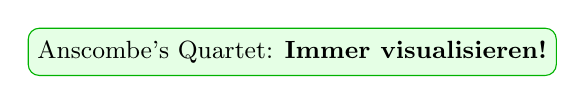
\begin{tikzpicture}
    \node[checklistbox] at (0,0) {Anscombe's Quartet: \textbf{Immer visualisieren!}};
\end{tikzpicture}
\end{center}
\end{frame}

\begin{frame}{Ausblick: Nächste Session}
\textbf{Session 12: Zeitreihenanalyse}

\begin{columns}[T]
\column{0.5\textwidth}
\textbf{Themen:}
\begin{itemize}
    \item Zeitreihenkomponenten
    \item Trend, Saisonalität, Residuen
    \item Window Functions: LAG, LEAD
    \item Moving Averages
    \item Year-over-Year Vergleiche
\end{itemize}

\column{0.5\textwidth}
\textbf{Vorbereitung:}
\begin{itemize}
    \item Session 9 (JOINs) wiederholen
    \item OVER-Klausel aus CTEs
\end{itemize}

\vspace{1em}
\begin{exampleblock}{Vorschau}
\texttt{LAG(sales, 12) OVER (ORDER BY month)}\\
$\rightarrow$ Wert vor 12 Monaten
\end{exampleblock}
\end{columns}
\end{frame}

\begin{frame}[plain]
\vfill
\begin{center}
{\Huge Fragen?}\\[2em]
{\Large\color{gray} christopher.flath@uni-wuerzburg.de}
\end{center}
\vfill
\end{frame}

\end{document}
